% Drawing 119/08-9 -- folder 119, batch 08, archive page 156 (PDF page 157).
% Transcription: deux ovales de 2 et 3 points
% Kind: two ovals of 2 and 3 points. Method 2 (schematic redraw from the facsimile). Status: ok.
% Notes: Two ovals, the first with points (one heavy) marked 2 below, the second with three points marked 3. The first oval seems to hold three marks (one large, two small) where the transcription counts 2; the label 2 is his.
% Coordinates: 1 unit = 1 mm = 1/100 of the crop width (bbox in page fractions: [0.17, 0.5, 0.4, 0.54]).
% Redrawn by Claude (claude-opus-5-5), issue #73, 2026-11-07; not checked by a human; not compiled (no TeX in the session).
% Rights: reproduces part of the work -- behind RENDER_TRANSCRIPTS, never published by itself.
\documentclass[tikz,border=3pt]{standalone}
\usepackage{amsmath,amssymb}
\usetikzlibrary{patterns,arrows.meta}
\tikzset{pencil/.style={black!45}, struck/.style={black!35}, mark/.style={circle,draw,inner sep=1.3pt}, pt/.style={circle,fill,inner sep=0.9pt}, opt/.style={circle,draw,fill=white,inner sep=1.1pt}}
\begin{document}
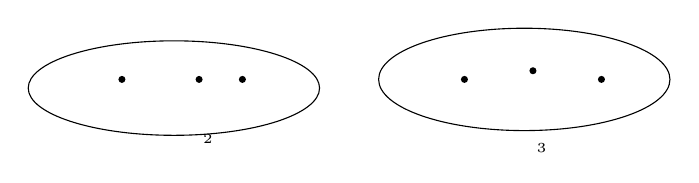
\begin{tikzpicture}[x=1mm,y=1mm,line cap=round,line join=round,font=\scriptsize]
\draw (28.3,-10.9) ellipse[x radius=18.5, y radius=6];
\node[pt] at (21.7,-9.8) {};
\node[pt] at (31.5,-9.8) {};
\node[pt] at (37,-9.8) {};
\node[inner sep=1pt] at (32.6,-17.4) {\tiny $2$};
\draw (72.8,-9.8) ellipse[x radius=18.5, y radius=6.5];
\node[pt] at (65.2,-9.8) {};
\node[pt] at (73.9,-8.7) {};
\node[pt] at (82.6,-9.8) {};
\node[inner sep=1pt] at (75,-18.5) {\tiny $3$};
\end{tikzpicture}
\end{document}
